\documentclass{article}
\usepackage{amsmath}
\usepackage{amssymb}
\usepackage{tikz}
\usetikzlibrary{3d}

\begin{document}

\begin{figure}[h]
    \centering
    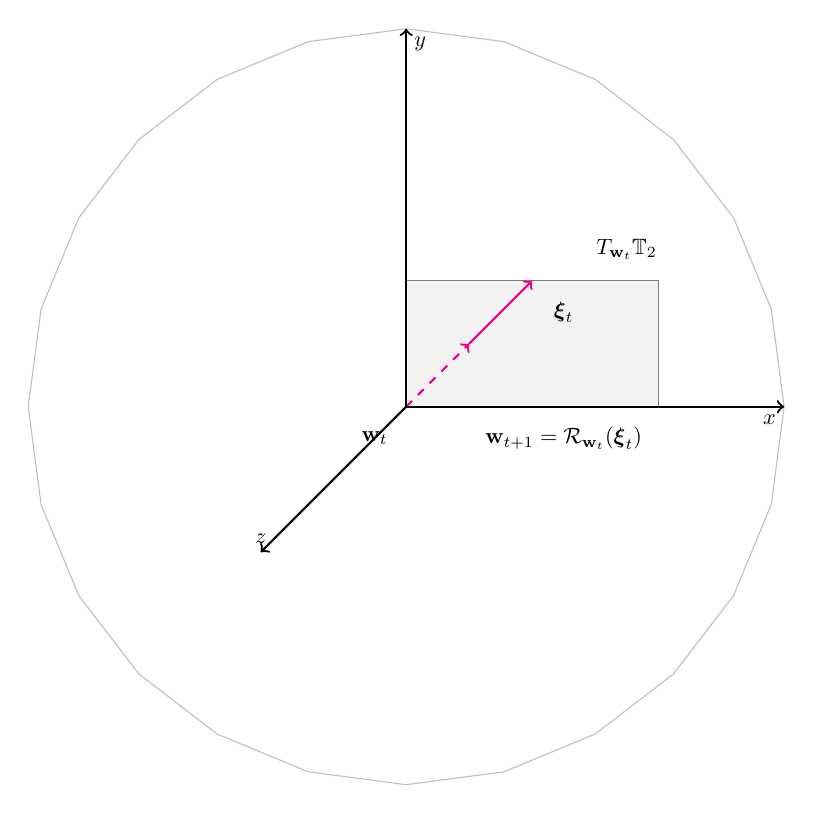
\begin{tikzpicture}[scale=0.8, transform shape, declare function={torusx(\u,\v)=6*cos(\u)*cos(\v); torusy(\u,\v)=6*sin(\u)*cos(\v); torusz(\u,\v)=6*sin(\v);}]
        % Torus surface
        \draw[gray!50, fill=gray!10] plot[domain=0:360, variable=\u] ({torusx(\u,0)}, {torusy(\u,0)}, {torusz(\u,0)}) -- plot[domain=0:360, variable=\u] ({torusx(\u,360)}, {torusy(\u,360)}, {torusz(\u,360)}) -- plot[domain=360:0, variable=\u] ({torusx(\u,360)}, {torusy(\u,360)}, {torusz(\u,360)}) -- plot[domain=360:0, variable=\u] ({torusx(\u,0)}, {torusy(\u,0)}, {torusz(\u,0)}) -- cycle;
        
        % Grid lines
        \foreach \u in {0,30,...,330}
            \draw[gray!50] ({torusx(\u,0)}, {torusy(\u,0)}, {torusz(\u,0)}) -- ({torusx(\u,360)}, {torusy(\u,360)}, {torusz(\u,360)});
        \foreach \v in {0,90,...,359}
            \draw[gray!50] ({torusx(0,\v)}, {torusy(0,\v)}, {torusz(0,\v)}) -- ({torusx(360,\v)}, {torusy(360,\v)}, {torusz(360,\v)});
        
        % Tangent plane
        \draw[fill=white!90!black, opacity=0.5] (0,0) -- (4,0) -- (4,2) -- (0,2) -- cycle;
        \draw[->, thick, dashed, magenta] (0,0) -- (1,1);
        \draw[->, thick, magenta] (1,1) -- (2,2);
        
        % Labels
        \node at (2.5,1.5) {$\boldsymbol{\xi}_t$};
        \node at (3.5,2.5) {$T_{\mathbf{w}_t}\mathbb{T}_2$};
        \node at (-0.5,-0.5) {$\mathbf{w}_t$};
        \node at (2.5,-0.5) {$\mathbf{w}_{t+1} = \mathcal{R}_{\mathbf{w}_t}(\boldsymbol{\xi}_t)$};
        
        % Axes
        \draw[->, thick] (0,0,0) -- (6,0,0) node[anchor=north east]{$x$};
        \draw[->, thick] (0,0,0) -- (0,6,0) node[anchor=north west]{$y$};
        \draw[->, thick] (0,0,0) -- (0,0,6) node[anchor=south]{$z$};
    \end{tikzpicture}
    \caption{Illustration of Riemannian optimization on $\mathbb{T}_2$ (represented as a torus embedded in $\mathbb{R}^3$): the iterate $\mathbf{w}_{t+1}$ is obtained from the retraction $\mathcal{R}_{\mathbf{w}_t}$ applied to the direction descent $\boldsymbol{\xi}_t \in T_{\mathbf{w}_t} \mathbb{T}_2$ (i.e., a vector of the tangent space of $\mathbb{T}_2$ at point $\mathbf{w}_t$).}
    \label{fig:riemannian_optimization_torus}
\end{figure}

\end{document}